\documentclass[a4paper]{report}

\usepackage[T1]{fontenc}
\usepackage[utf8]{inputenc}
\usepackage[english]{babel}

\usepackage{booktabs}
\renewcommand{\arraystretch}{1.2}

% Display code - main interest is it can import external files
\usepackage{listings}
\usepackage[usenames]{xcolor}

% Custom style for the code
\lstset{
	commentstyle=\color{gray},
	tabsize=4,
	basicstyle={\small\ttfamily}
}

% TiKZ for the drawings
\usepackage{tikz}
\usetikzlibrary{shapes}

\setlength{\textwidth}{16cm} \setlength{\textheight}{23cm}
\setlength{\oddsidemargin}{0cm} % +0.5 si {\textwidth}{15cm} ; -0,5 si {\textwidth}{15cm}
\setlength{\headheight}{0cm} \setlength{\topmargin}{0.3cm}
\setlength{\headsep}{0cm}

% Deletes the chapters and uses roman numbers for the sections
\usepackage{chngcntr}
\counterwithout{section}{section}
\renewcommand{\thesection}{\Roman{section}}
\renewcommand{\thesubsection}{\thesection.\arabic{subsection}}
\renewcommand{\thesubsubsection}{\thesection.\arabic{subsection}.\alph{subsubsection}}

\usepackage{mathtools} % Allows to write \textwidth-2cm in \includegraphics

\author{Clément Decoodt, Alexis Bauvin, Alexandre Janniaux}
\title{PR2 SE201: execution platforms}

\begin{document}

\maketitle

\section{Introduction}

In this report, we will detail our results on the analysis of MIPS code execution.

\section{Warm up}

Nothing to do here

\section{Pipeline}

There are many clues which show the processor is enabled to forwarding.

First, the statistics window tell us:
\begin{verbatim}
ALU forwarded values: 2 (from execute: 2, memory stage: 0, write back: 0)
\end{verbatim}

Then, the log window tells us, for instruction 13:
\begin{verbatim}
DEBUG [EXECUTE]: {FW} PC: 0x000011a0 forwarding changed value for ALU port A RS from:
0x0 to: 0xffffffe0
\end{verbatim}

But we can also tell that the processor does forward because of the pipeline window.
Indeed, the processor compute the following instructions:

\begin{verbatim}
    1. nop
    2. addui r29,r29,-32
    3. sw 28(r29),r31
    4. sw 24(r29),r30
    5. or r30,r29,r0
\end{verbatim}

So instruction $3.$ and $4.$  depends on instruction $2.$ which is executed at cycle $12$.
At instruction $13$, $12$ has been executed, but the result is not written back in register yet,
and $3.$ is to be decoded. It means that $3.$ is able to use the result from $2.$ before $2.$ has finished
to store his value.

\begin{center}
	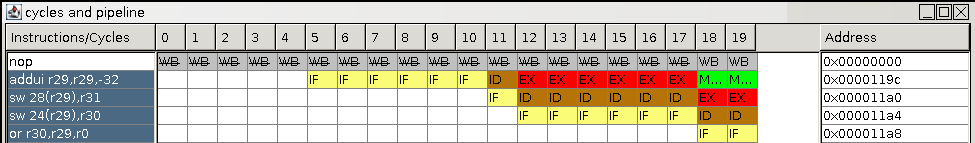
\includegraphics[width=\textwidth-2cm]{images/pipeline_forwarding.png}
\end{center}

There are such unfinished instructions in the following screenshot :

\begin{center}
	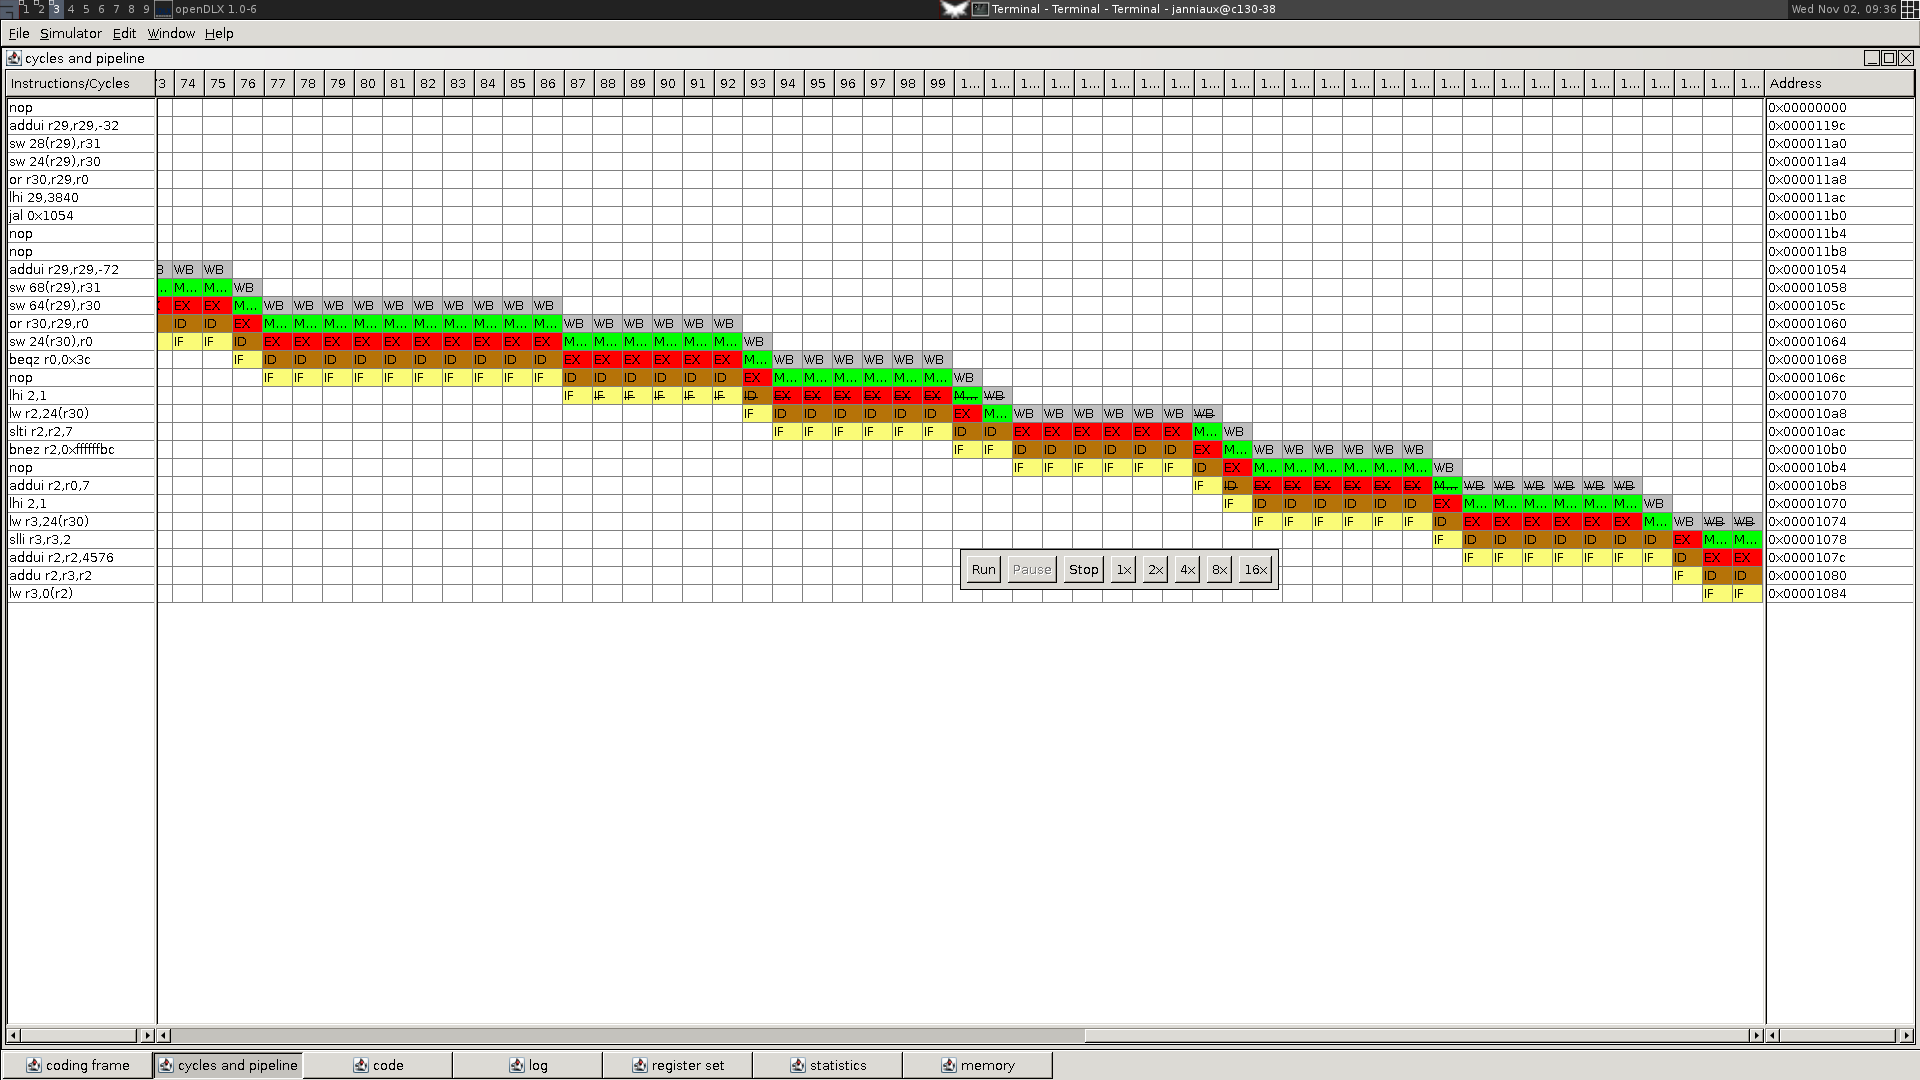
\includegraphics[width=\textwidth-2cm]{images/pipeline_no_writeback_after_branching.png}
\end{center}

Here we can see that the \texttt{lhi 2,1} instruction never reaches the WB stage. This is because the
\texttt{beqz~r0,0x3c} was mispredicted, thus the instruction is flushed, discarding its result.

\begin{center}
	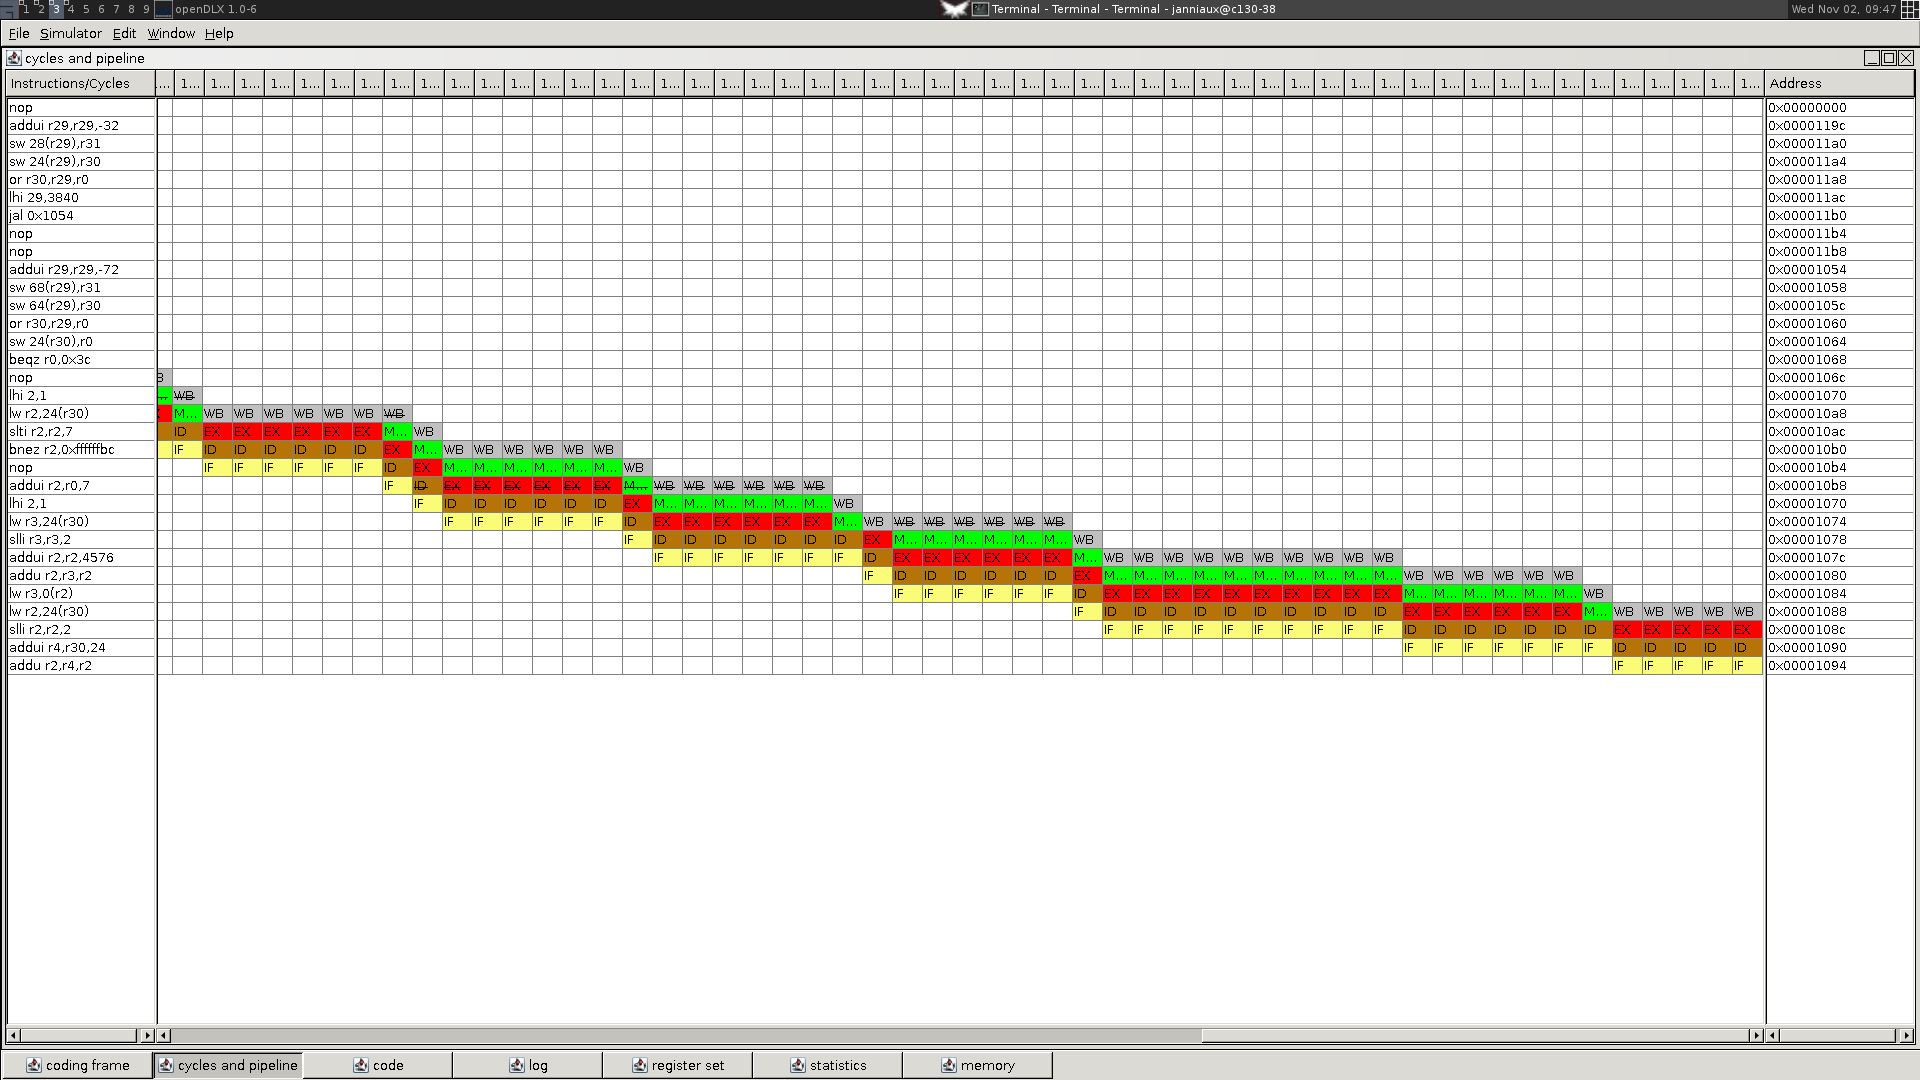
\includegraphics[width=\textwidth-2cm]{images/pipeline_no_writeback_after_forwarding.png}
\end{center}

In this part, we see that the \texttt{lw~r3,24(r30)} is not written back to the registers because its output
register, \texttt{r3}, is reused by the next instruction as an input and an output. Thus the value stays in
the pipeline because it is forwarded, it would be erased otherwise.
\mbox{}\\

Overall we notice that all branches are handled the same way : branch instructions are followed by a
\texttt{nop} that is fully executed, then by another instruction that is discarded (flushed). This is because
the branch predictor needs a full cycle to tell wether it mispredicted.

\section{Branch prediction}

The useful statistics are provided in the \texttt{rates.log} file, containing stats for both 1-bit and 2-bit
branch predictor. Overall, the 2-bit predictor saved us 4 cycles over the 1-bit predictor and lowered the
misprediction rate from 19,14\% to 18,09\%. Although the benefits look small, they are instresting as a 2-bit
saturation predictor is rather simple logic.

It is important to note that, following an update of openDLX, the total jump count is lower in the 2-bit
simulation than in the 1-bit one.
\mbox{}\\

The BPC stats are in the \texttt{bpc.log} file. Only lines 2 and 3 do differ between the 1-bit and the 2-bit
BPC. Although the second branch is a bit worse with a misprediction rate of 0,22 compared to the ratio of 0,16
(37.5\% worsening) of the 1-bit BPC, the third branch is ways better with a rate of 0,26 instead of 0,44
(59\% improvement). Overall, the 2-bit BPC is better.

\end{document}


